\newpage
\section{A/D-D/A Umsetzereinheit}

\subsection{Aufgabenstellung}

Der Ausgang des Flash Converters wird mit dem Digital Analog umsetzer verbunden, um das digitale Signal zu beobachten und die unterschiede festzustellen. Es soll speziell der Quantisierungssfehler und das Verhalten bei höhereren Frequenzen untersucht werden.

\subsection{Versuchsaufbau}

Am Flash Converter wird das Fehlerprogramm 2 eingestellt. Das Taktsignal des Flash Converters und der Anzeige wird mit $n\cdot CLK$ verbunden. Der Eingang wird mit dem Funktionsgenerator verbunden. $U_\mathrm{a}$ und $U_\mathrm{e}$ werden am Oszilloskop dargestellt. Der Versuchsaufbau ist in Abbildung \ref{fig:20-ad-da-schaltung} dargestellt.

\begin{figure}[h]
	\centering
	
\includegraphics[width=0.7\textwidth]{images/20_AD-DA_Schaltung.png}	
	\caption{Versuchsaufbau A/D - D/A Umsetzer}\label{fig:20-ad-da-schaltung}	
\end{figure}

\subsection{Quantisierungsfehler}

\begin{wrapfigure}[11]{r}{0.4\textwidth}
	\centering
	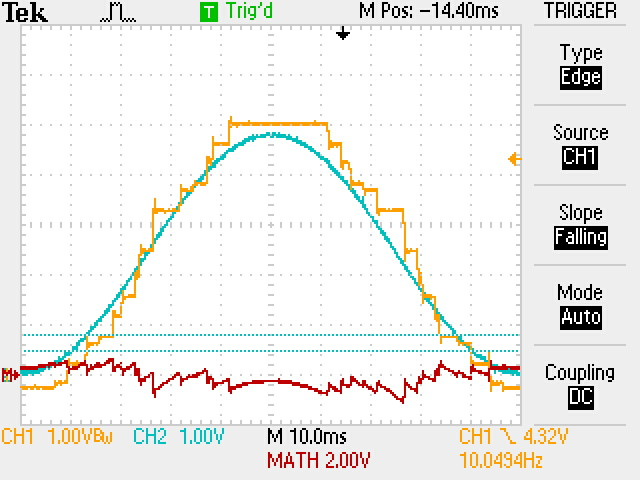
\includegraphics[width=0.4\textwidth]{images/21_Flash_Quantisierung.JPG}	
	\captionof{figure}{Darstellung des Quantisierten Signals.\\ CH1 $U_\mathrm{e}$, CH2 $U_\mathrm{a}$, MATH $F_Q$}\label{fig:20-dac-curve}	
\end{wrapfigure}

Am Eingang des Flashconverters $U_\mathrm{e}$ wird eine Sinusspannung mit $\SI{5}{\volt}_{pp}$ und \SI{10}{\hertz} mit dem Funktionsgenerator eingestellt. Um den Quantisierungsfehler zu beobachten wird zunächst die Eingangsspannung $U_\mathrm{e}$ und die Ausgangsspannung $U_\mathrm{a}$ des D/A Umsetzers auf dem Oszilloskop dargestellt. Danach wird die Quantisierungsfehler $F_Q = U_\mathrm{e} - U_\mathrm{a}$ mit der \textit{Math}-Funktion am Oszilloskop berechnet und in Abbildung \ref{fig:20-dac-curve} dargestellt.

Zu erkennen ist dass das Ausgangssignal nicht mehr Wertkontinuierlich ist, da mit der Auflösung der Wandler nur eine endliche Anzahl an Spannungswerten dargestellt werden kann. Die zu sehenden Stufen sorgen für eine Abweichung des Ausgangssignals zum Eingangssignal, welche als Quantisierungsfehler bezeichnet wird.

\subsection{Frequenzverhalten}

Nun wird die Frequenz der Sinusspannung am Eingang $U_\mathrm{e}$ erhöht. Dabei werden die Frequenzen \SI{10}{\hertz}, \SI{100}{\hertz} und \SI{1}{\kilo\hertz} gewählt und das Ausgangssignal $U_\mathrm{a}$ des D/A Umsetzers beobachtet. Die Ergebnisse sind in Abbildung \ref{fig:20-dac-freq} dargestellt.

\begin{figure}[h]
	\begin{minipage}[t]{0.3\textwidth}
	\centering
	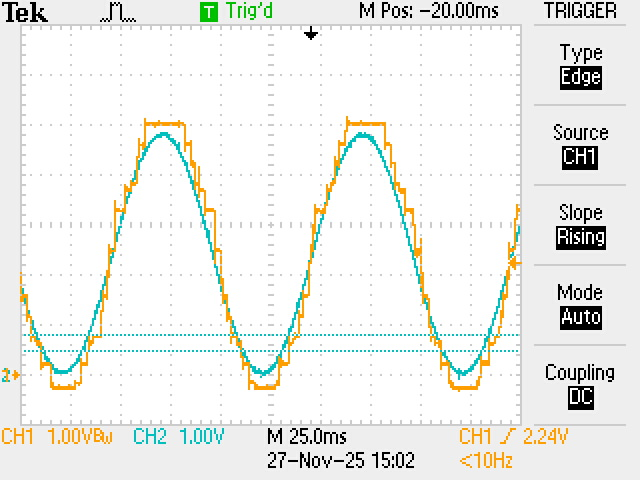
\includegraphics[width=\textwidth]{images/20_Flash_10Hz.JPG}	
	\caption*{(a) $f = \SI{10}{\hertz}$}\label{fig:dac-10Hz}	
	\end{minipage}\hfill
	\begin{minipage}[t]{0.3\textwidth}
	\centering
	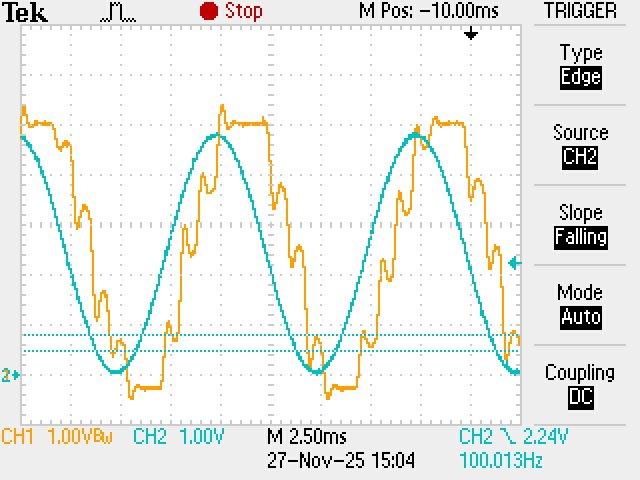
\includegraphics[width=\textwidth]{images/20_Flash_100Hz.JPG}	
	\caption*{(b) $f = \SI{100}{\hertz}$}\label{fig:dac-100Hz}	
	\end{minipage}\hfill
	\begin{minipage}[t]{0.3\textwidth}
	\centering
	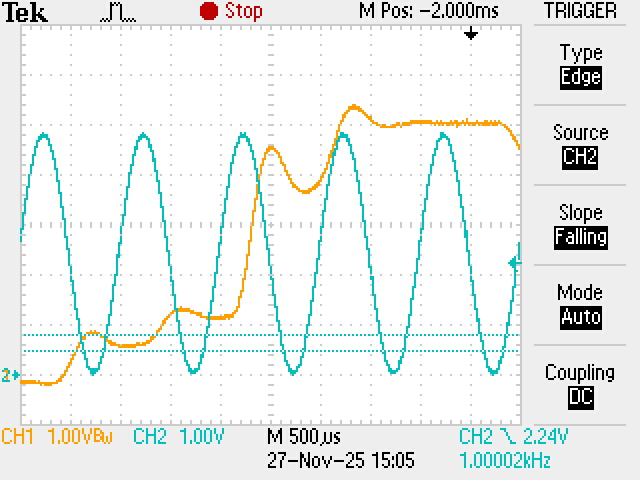
\includegraphics[width=\textwidth]{images/20_Flash_1000Hz.JPG}	
	\caption*{(c) $f = \SI{1}{\kilo\hertz}$}\label{fig:dac-1kHz}	
	\end{minipage}
	\caption{Frequenzverhalten des D/A Umsetzers bei verschiedenen Eingangssignalfrequenzen}\label{fig:20-dac-freq}
\end{figure}

Zu erkennen ist, dass bei höheren Frequenzen das Ausgangssignal des D/A Umsetzers zunehmend verzerrt wird. Der Grund dafür ist, dass Signal nur begrenzt schnell genug mit dem $n\cdot CLK$-Taktsignal abgetastet wird und ab einer bestimmten Frequenz das Abtasttheorem $f_\mathrm{sig,max} = f_\mathrm{Sample} / 2$ verletzt. Für $n\cdot CLK=\SI{1800}{\hertz}$ ist die maximale Signalfrequenz $f_\mathrm{sig,max} = \SI{900}{\hertz}$. Man erkennt in \autoref{fig:20-dac-freq} (c), dass bei dieser Frequenz das Signal nicht mehr korrekt rekonstruiert werden kann.